\title{2016 年高考数学 全国I卷-文科}
\date{}
\maketitle

\section*{一、选择题}
本大题共12小题，每小题5分，在每小题给出的四个选项中，只有一项是符合题目要求的。

\begin{question}[points=5]
设集合$A=\{1,3,5,7\}$，$B=\{x|2\le x\le5\}$，则$A\cap B=$
\begin{choices}
  \item $\{1,3\}$
  \item $\{3,5\}$
  \item $\{5,7\}$
  \item $\{1,7\}$
\end{choices}
\begin{solution}
\textbf{答案：}$\{3,5\}$

\textbf{分析：}直接利用交集的运算法则化简求解即可。

\textbf{详解：}集合$A=\{1,3,5,7\}$，$B=\{x|2\le x\le5\}$，则$A\cap B=\{3,5\}$。故选：$B$。
\end{solution}
\end{question}

\begin{question}[points=5]
设$(1+2i)(a+i)$的实部与虚部相等，其中$a$为实数，则$a$等于
\begin{choices}
  \item $-3$
  \item $-2$
  \item $2$
  \item $3$
\end{choices}
\begin{solution}
\textbf{答案：}$-3$

\textbf{分析：}利用复数的乘法运算法则，通过复数相等的充要条件求解即可。

\textbf{详解：}$(1+2i)(a+i)=a-2+(2a+1)i$的实部与虚部相等，可得$a-2=2a+1$，解得$a=-3$。故选：$A$。
\end{solution}
\end{question}

\begin{question}[points=5]
为美化环境，从红、黄、白、紫4种颜色的花中任选2种花种在一个花坛中，余下的2种花种在另一个花坛中，则红色和紫色的花不在同一花坛的概率是
\begin{choices}
  \item $\frac{1}{3}$
  \item $\frac{1}{2}$
  \item $\frac{2}{3}$
  \item $\frac{5}{6}$
\end{choices}
\begin{solution}
\textbf{答案：}$\frac{2}{3}$

\textbf{分析：}确定基本事件的个数，利用古典概型的概率公式，可得结论。

\textbf{详解：}从红、黄、白、紫4种颜色的花中任选2种花种在一个花坛中，余下的2种花种在另一个花坛中，有$C_4^2=6$种方法，红色和紫色的花在同一花坛，有2种方法，红色和紫色的花不在同一花坛，有4种方法，所以所求的概率为$\frac{4}{6}=\frac{2}{3}$。故选：$C$。
\end{solution}
\end{question}

\begin{question}[points=5]
$\triangle ABC$的内角$A$、$B$、$C$的对边分别为$a$、$b$、$c$。已知$a=\sqrt{5}$，$c=2$，$\cos A=\frac{2}{3}$，则$b=$
\begin{choices}
  \item $\sqrt{2}$
  \item $\sqrt{3}$
  \item $2$
  \item $3$
\end{choices}
\begin{solution}
\textbf{答案：}$3$

\textbf{分析：}由余弦定理可得$\cos A=\frac{b^2+c^2-a^2}{2bc}$，利用已知整理可得$3b^2-8b-3=0$，从而解得$b$的值。

\textbf{详解：}$\because a=\sqrt{5}$，$c=2$，$\cos A=\frac{2}{3}$，$\therefore$由余弦定理可得：$\cos A=\frac{b^2+c^2-a^2}{2bc}=\frac{b^2+4-5}{4b}=\frac{b^2-1}{4b}=\frac{2}{3}$，整理可得：$3b^2-8b-3=0$，$\therefore$解得：$b=3$或$-\frac{1}{3}$（舍去）。故选：$D$。
\end{solution}
\end{question}

\begin{question}[points=5]
直线$l$经过椭圆的一个顶点和一个焦点，若椭圆中心到$l$的距离为其短轴长的$\frac{1}{4}$，则该椭圆的离心率为
\begin{choices}
  \item $\frac{1}{3}$
  \item $\frac{1}{2}$
  \item $\frac{2}{3}$
  \item $\frac{3}{4}$
\end{choices}
\begin{solution}
\textbf{答案：}$\frac{1}{2}$

\textbf{分析：}设出椭圆的方程，求出直线的方程，利用已知条件列出方程，即可求解椭圆的离心率。

\textbf{详解：}设椭圆的方程为$\frac{x^2}{a^2}+\frac{y^2}{b^2}=1$，直线$l$经过椭圆的一个顶点$(0,b)$和一个焦点$(c,0)$，则直线方程为$\frac{x}{c}+\frac{y}{b}=1$，椭圆中心到$l$的距离为其短轴长的$\frac{1}{4}$，可得$\frac{1}{\sqrt{\frac{1}{c^2}+\frac{1}{b^2}}}=\frac{2b}{4}$，$\therefore \frac{bc}{\sqrt{b^2+c^2}}=\frac{b}{2}$，$\therefore \frac{c}{\sqrt{b^2+c^2}}=\frac{1}{2}$，$\therefore \frac{c^2}{a^2}=\frac{1}{4}$，$\therefore e=\frac{c}{a}=\frac{1}{2}$。故选：$B$。
\end{solution}
\end{question}

\begin{question}[points=5]
将函数$y=2\sin(2x+\frac{\pi}{6})$的图象向右平移$\frac{1}{4}$个周期后，所得图象对应的函数为
\begin{choices}
  \item $y=2\sin(2x+\frac{\pi}{4})$
  \item $y=2\sin(2x+\frac{\pi}{3})$
  \item $y=2\sin(2x-\frac{\pi}{4})$
  \item $y=2\sin(2x-\frac{\pi}{3})$
\end{choices}
\begin{solution}
\textbf{答案：}$y=2\sin(2x-\frac{\pi}{3})$

\textbf{分析：}求得函数$y$的最小正周期，即有所对的函数式为$y=2\sin[2(x-\frac{\pi}{4})+\frac{\pi}{6}]$，化简整理即可得到所求函数式。

\textbf{详解：}函数$y=2\sin(2x+\frac{\pi}{6})$的周期为$T=\frac{2\pi}{2}=\pi$，由题意即为函数$y=2\sin(2x+\frac{\pi}{6})$的图象向右平移$\frac{\pi}{4}$个单位，可得图象对应的函数为$y=2\sin[2(x-\frac{\pi}{4})+\frac{\pi}{6}]$，即有$y=2\sin(2x-\frac{\pi}{3})$。故选：$D$。
\end{solution}
\end{question}

\begin{question}[points=5]
如图，某几何体的三视图是三个半径相等的圆及每个圆中两条相互垂直的半径。若该几何体的体积是$\frac{28\pi}{3}$，则它的表面积是
\begin{choices}
  \item $17\pi$
  \item $18\pi$
  \item $20\pi$
  \item $28\pi$
\end{choices}
\begin{solution}
\textbf{答案：}$17\pi$

\textbf{分析：}判断三视图复原的几何体的形状，利用体积求出几何体的半径，然后求解几何体的表面积。

\textbf{详解：}由题意可知三视图复原的几何体是一个球去掉$\frac{1}{8}$后的几何体，如图：可得：$\frac{7}{8}\times\frac{4}{3}\pi R^3=\frac{28\pi}{3}$，$R=2$。它的表面积是：$\frac{7}{8}\times4\pi\cdot2^2+\frac{3}{4}\times\pi\cdot2^2=17\pi$。故选：$A$。
\end{solution}
\end{question}

\begin{question}[points=5]
若$a>b>0$，$0<c<1$，则
\begin{choices}
  \item $\log_ac<\log_bc$
  \item $\log_ca<\log_cb$
  \item $a^c<b^c$
  \item $c^a>c^b$
\end{choices}
\begin{solution}
\textbf{答案：}$\log_ca<\log_cb$

\textbf{分析：}根据指数函数，对数函数，幂函数的单调性结合换底公式，逐一分析四个结论的真假，可得答案。

\textbf{详解：}$\because a>b>0$，$0<c<1$，$\therefore \log_ca<\log_cb$，故$B$正确；$\therefore$当$a>b>1$时，$0>\log_ac>\log_bc$，故$A$错误；$a^c>b^c$，故$C$错误；$c^a<c^b$，故$D$错误。故选：$B$。
\end{solution}
\end{question}

\begin{question}[points=5]
函数$y=2x^2-e^{|x|}$在$[-2,2]$的图象大致为
\begin{choices}
\end{choices}
\begin{solution}
\textbf{答案：}$D$

\textbf{分析：}根据已知中函数的解析式，分析函数的奇偶性，最大值及单调性，利用排除法，可得答案。

\textbf{详解：}$\because f(x)=y=2x^2-e^{|x|}$，$\therefore f(-x)=2(-x)^2-e^{|-x|}=2x^2-e^{|x|}$，故函数为偶函数，当$x=\pm2$时，$y=8-e^2\in(0,1)$，故排除$A$，$B$；当$x\in[0,2]$时，$f(x)=y=2x^2-e^x$，$\therefore f'(x)=4x-e^x=0$有解，故函数$y=2x^2-e^{|x|}$在$[0,2]$不是单调的，故排除$C$，故选：$D$。
\end{solution}
\end{question}

\begin{question}[points=5]
执行下面的程序框图，如果输入的$x=0$，$y=1$，$n=1$，则输出$x$，$y$的值满足
\begin{choices}
  \item $y=2x$
  \item $y=3x$
  \item $y=4x$
  \item $y=5x$
\end{choices}
\begin{solution}
\textbf{答案：}$y=4x$

\textbf{分析：}由已知中的程序框图可知：该程序的功能是利用循环结构计算并输出变量$x$，$y$的值，模拟程序的运行过程，分析循环中各变量值的变化情况，可得答案。

\textbf{详解：}输入$x=0$，$y=1$，$n=1$，则$x=0$，$y=1$，不满足$x^2+y^2\ge36$，故$n=2$，则$x=\frac{1}{2}$，$y=2$，不满足$x^2+y^2\ge36$，故$n=3$，则$x=\frac{3}{2}$，$y=6$，满足$x^2+y^2\ge36$，故$y=4x$，故选：$C$。
\end{solution}
\end{question}

\begin{question}[points=5]
平面$\alpha$过正方体$ABCD-A_1B_1C_1D_1$的顶点$A$，$\alpha\parallel$平面$CB_1D_1$，$\alpha\cap$平面$ABCD=m$，$\alpha\cap$平面$ABB_1A_1=n$，则$m$、$n$所成角的正弦值为
\begin{choices}
  \item $\frac{\sqrt{3}}{2}$
  \item $\frac{\sqrt{2}}{2}$
  \item $\frac{\sqrt{3}}{3}$
  \item $\frac{1}{3}$
\end{choices}
\begin{solution}
\textbf{答案：}$\frac{\sqrt{3}}{2}$

\textbf{分析：}画出图形，判断出$m$、$n$所成角，求解即可。

\textbf{详解：}如图：$\alpha\parallel$平面$CB_1D_1$，$\alpha\cap$平面$ABCD=m$，$\alpha\cap$平面$ABA_1B_1=n$，可知：$n\parallel CD_1$，$m\parallel B_1D_1$，$\because \triangle CB_1D_1$是正三角形。$m$、$n$所成角就是$\angle CD_1B_1=60^\circ$。则$m$、$n$所成角的正弦值为：$\sin60^\circ=\frac{\sqrt{3}}{2}$。故选：$A$。
\end{solution}
\end{question}

\begin{question}[points=5]
若函数$f(x)=x-\frac{1}{3}\sin2x+a\sin x$在$(-\infty,+\infty)$单调递增，则$a$的取值范围是
\begin{choices}
  \item $[-1,1]$
  \item $[-1,\frac{1}{3}]$
  \item $[-\frac{1}{3},\frac{1}{3}]$
  \item $[-1,-\frac{1}{3}]$
\end{choices}
\begin{solution}
\textbf{答案：}$[-\frac{1}{3},\frac{1}{3}]$

\textbf{分析：}求出$f(x)$的导数，由题意可得$f'(x)\ge0$恒成立，设$t=\cos x(-1\le t\le1)$，即有$5-4t^2+3at\ge0$，对$t$讨论，分$t=0$，$0<t\le1$，$-1\le t<0$，分离参数，运用函数的单调性可得最值，解不等式即可得到所求范围。

\textbf{详解：}函数$f(x)=x-\frac{1}{3}\sin2x+a\sin x$的导数为$f'(x)=1-\frac{2}{3}\cos2x+a\cos x$，由题意可得$f'(x)\ge0$恒成立，即为$1-\frac{2}{3}\cos2x+a\cos x\ge0$，即有$\frac{5}{3}-\frac{4}{3}\cos^2x+a\cos x\ge0$，设$t=\cos x(-1\le t\le1)$，即有$5-4t^2+3at\ge0$，当$t=0$时，不等式显然成立；当$0<t\le1$时，$3a\ge4t-\frac{5}{t}$，由$4t-\frac{5}{t}$在$(0,1]$递增，可得$t=1$时，取得最大值$-1$，可得$3a\ge-1$，即$a\ge-\frac{1}{3}$；当$-1\le t<0$时，$3a\le4t-\frac{5}{t}$，由$4t-\frac{5}{t}$在$[-1,0)$递增，可得$t=-1$时，取得最小值$1$，可得$3a\le1$，即$a\le\frac{1}{3}$。综上可得$a$的范围是$[-\frac{1}{3},\frac{1}{3}]$。另解：设$t=\cos x(-1\le t\le1)$，即有$5-4t^2+3at\ge0$，由题意可得$5-4+3a\ge0$，且$5-4-3a\ge0$，解得$a$的范围是$[-\frac{1}{3},\frac{1}{3}]$。故选：$C$。
\end{solution}
\end{question}

\section*{二、填空题}
本大题共4小题，每小题5分。

\begin{question}[points=5]
设向量$\vec{a}=(x,x+1)$，$\vec{b}=(1,2)$，且$\vec{a}\perp\vec{b}$，则$x=$
\fillin[{$-\frac{2}{3}$}]
\begin{solution}
\textbf{答案：}$-\frac{2}{3}$

\textbf{分析：}根据向量垂直的充要条件便可得出$\vec{a}\cdot\vec{b}=0$，进行向量数量积的坐标运算即可得出关于$x$的方程，解方程便可得出$x$的值。

\textbf{详解：}$\because \vec{a}\perp\vec{b}$；$\therefore \vec{a}\cdot\vec{b}=0$；即$x+2(x+1)=0$；$\therefore x=-\frac{2}{3}$。故答案为：$-\frac{2}{3}$。
\end{solution}
\end{question}

\begin{question}[points=5]
已知$\theta$是第四象限角，且$\sin(\theta+\frac{\pi}{4})=\frac{3}{5}$，则$\tan(\theta-\frac{\pi}{4})=$
\fillin[{$-\frac{4}{3}$}]
\begin{solution}
\textbf{答案：}$-\frac{4}{3}$

\textbf{分析：}由$\theta$得范围求得$\theta+\frac{\pi}{4}$的范围，结合已知求得$\cos(\theta+\frac{\pi}{4})$，再由诱导公式求得$\sin(\frac{\pi}{4}-\theta)$及$\cos(\frac{\pi}{4}-\theta)$，进一步由诱导公式及同角三角函数基本关系式求得$\tan(\theta-\frac{\pi}{4})$的值。

\textbf{详解：}$\because\theta$是第四象限角，$\therefore -\frac{\pi}{2}+2k\pi<\theta<2k\pi$，则$-\frac{\pi}{4}+2k\pi<\theta+\frac{\pi}{4}<\frac{\pi}{4}+2k\pi$，又$\sin(\theta+\frac{\pi}{4})=\frac{3}{5}$，$\therefore\cos(\theta+\frac{\pi}{4})=\frac{4}{5}$。$\therefore\cos(\frac{\pi}{4}-\theta)=\sin(\theta+\frac{\pi}{4})=\frac{3}{5}$，$\sin(\frac{\pi}{4}-\theta)=\cos(\theta+\frac{\pi}{4})=\frac{4}{5}$。则$\tan(\theta-\frac{\pi}{4})=-\tan(\frac{\pi}{4}-\theta)=-\frac{\sin(\frac{\pi}{4}-\theta)}{\cos(\frac{\pi}{4}-\theta)}=-\frac{4}{3}$。故答案为：$-\frac{4}{3}$。
\end{solution}
\end{question}

\begin{question}[points=5]
设直线$y=x+2a$与圆$C:x^2+y^2-2ay-2=0$相交于$A$，$B$两点，若$|AB|=2\sqrt{3}$，则圆$C$的面积为
\fillin[{$4\pi$}]
\begin{solution}
\textbf{答案：}$4\pi$

\textbf{分析：}圆$C:x^2+y^2-2ay-2=0$的圆心坐标为$(0,a)$，半径为$\sqrt{a^2+2}$，利用圆的弦长公式，求出$a$值，进而求出圆半径，可得圆的面积。

\textbf{详解：}圆$C:x^2+y^2-2ay-2=0$的圆心坐标为$(0,a)$，半径为$\sqrt{a^2+2}$，$\because$直线$y=x+2a$与圆$C$相交于$A$，$B$两点，且$|AB|=2\sqrt{3}$，$\therefore$圆心$(0,a)$到直线$y=x+2a$的距离$d=\frac{|0-a+2a|}{\sqrt{2}}=\frac{|a|}{\sqrt{2}}$，即$(\frac{|a|}{\sqrt{2}})^2+(\sqrt{3})^2=a^2+2$，解得：$a^2=2$，故圆的半径$r=2$。故圆的面积$S=4\pi$，故答案为：$4\pi$。
\end{solution}
\end{question}

\begin{question}[points=5]
某高科技企业生产产品$A$和产品$B$需要甲、乙两种新型材料。生产一件产品$A$需要甲材料$1.5\text{kg}$，乙材料$1\text{kg}$，用$5$个工时；生产一件产品$B$需要甲材料$0.5\text{kg}$，乙材料$0.3\text{kg}$，用$3$个工时，生产一件产品$A$的利润为$2100$元，生产一件产品$B$的利润为$900$元。该企业现有甲材料$150\text{kg}$，乙材料$90\text{kg}$，则在不超过$600$个工时的条件下，生产产品$A$、产品$B$的利润之和的最大值为
\fillin[{$216000$}]
\begin{solution}
\textbf{答案：}$216000$

\textbf{分析：}设$A$、$B$两种产品分别是$x$件和$y$件，根据题干的等量关系建立不等式组以及目标函数，利用线性规划作出可行域，通过目标函数的几何意义，求出其最大值即可。

\textbf{详解：}设$A$、$B$两种产品分别是$x$件和$y$件，获利为$z$元。由题意，得$\begin{cases} 1.5x+0.5y\le150 \\ x+0.3y\le90 \\ 5x+3y\le600 \\ x\ge0,y\ge0 \end{cases}$，$z=2100x+900y$。不等式组表示的可行域如图：由题意可得$\begin{cases} x+0.3y=90 \\ 5x+3y=600 \end{cases}$，解得：$\begin{cases} x=60 \\ y=100 \end{cases}$，$A(60,100)$，目标函数$z=2100x+900y$。经过$A$时，直线的截距最大，目标函数取得最大值：$2100\times60+900\times100=216000$元。故答案为：$216000$。
\end{solution}
\end{question}

\section*{三、解答题}
解答应写出文字说明，证明过程或演算步骤。

\begin{question}[points=12]
已知$\{a_n\}$是公差为3的等差数列，数列$\{b_n\}$满足$b_1=1$，$b_2=\frac{1}{3}$，$a_nb_{n+1}+b_{n+1}=nb_n$。

（Ⅰ）求$\{a_n\}$的通项公式；

（Ⅱ）求$\{b_n\}$的前$n$项和。
\begin{solution}
\textbf{答案：}（Ⅰ）$a_n=3n-1$；（Ⅱ）$S_n=\frac{3}{2}(1-3^{-n})=\frac{3}{2}-\frac{1}{2\cdot3^{n-1}}$

\textbf{分析：}（Ⅰ）令$n=1$，可得$a_1=2$，结合$\{a_n\}$是公差为3的等差数列，可得$\{a_n\}$的通项公式；
（Ⅱ）由（Ⅰ）可得：数列$\{b_n\}$是以1为首项，以$\frac{1}{3}$为公比的等比数列，进而可得$\{b_n\}$的前$n$项和。

\textbf{详解：}（Ⅰ）$\because a_nb_{n+1}+b_{n+1}=nb_n$。当$n=1$时，$a_1b_2+b_2=b_1$。$\because b_1=1$，$b_2=\frac{1}{3}$，$\therefore a_1=2$，又$\because \{a_n\}$是公差为3的等差数列，$\therefore a_n=3n-1$。
（Ⅱ）由（I）知：$(3n-1)b_{n+1}+b_{n+1}=nb_n$，即$3b_{n+1}=b_n$。即数列$\{b_n\}$是以1为首项，以$\frac{1}{3}$为公比的等比数列，$\therefore \{b_n\}$的前$n$项和$S_n=\frac{1\times(1-(\frac{1}{3})^n)}{1-\frac{1}{3}}=\frac{3}{2}(1-3^{-n})=\frac{3}{2}-\frac{1}{2\cdot3^{n-1}}$。
\end{solution}
\end{question}

\begin{question}[points=12]
如图，已知正三棱锥$P-ABC$的侧面是直角三角形，$PA=6$，顶点$P$在平面$ABC$内的正投影为点$D$，$D$在平面$PAB$内的正投影为点$E$，连接$PE$并延长交$AB$于点$G$。

（Ⅰ）证明：$G$是$AB$的中点；

（Ⅱ）在图中作出点$E$在平面$PAC$内的正投影$F$（说明作法及理由），并求四面体$PDEF$的体积。

\begin{center}
  
\includegraphics[width=.38\linewidth]{question-18-1.jpg}
\end{center}
\begin{solution}
\textbf{答案：}（Ⅰ）证明见解析；（Ⅱ）作图见解析，$V_{PDEF}=\frac{4}{3}$

\textbf{分析：}（Ⅰ）根据题意分析可得$PD\perp$平面$ABC$，进而可得$PD\perp AB$，同理可得$DE\perp AB$，结合两者分析可得$AB\perp$平面$PDE$，进而分析可得$AB\perp PG$，又由$PA=PB$，由等腰三角形的性质可得证明；
（Ⅱ）由线面垂直的判定方法可得$EF\perp$平面$PAC$，可得$F$为$E$在平面$PAC$内的正投影。由棱锥的体积公式计算可得答案。

\textbf{详解：}（Ⅰ）证明：$\because P-ABC$为正三棱锥，且$D$为顶点$P$在平面$ABC$内的正投影，$\therefore PD\perp$平面$ABC$，则$PD\perp AB$，又$E$为$D$在平面$PAB$内的正投影，$\therefore DE\perp$面$PAB$，则$DE\perp AB$，$\because PD\cap DE=D$，$\therefore AB\perp$平面$PDE$，连接$PE$并延长交$AB$于点$G$，则$AB\perp PG$，又$PA=PB$，$\therefore G$是$AB$的中点；
（Ⅱ）在平面$PAB$内，过点$E$作$PB$的平行线交$PA$于点$F$，$F$即为$E$在平面$PAC$内的正投影。$\because$正三棱锥$P-ABC$的侧面是直角三角形，$\therefore PB\perp PA$，$PB\perp PC$，又$EF\parallel PB$，所以$EF\perp PA$，$EF\perp PC$，因此$EF\perp$平面$PAC$，即点$F$为$E$在平面$PAC$内的正投影。连结$CG$，因为$P$在平面$ABC$内的正投影为$D$，所以$D$是正三角形$ABC$的中心。由（Ⅰ）知，$G$是$AB$的中点，所以$D$在$CG$上，故$CD=\frac{2}{3}CG$。由题设可得$PC\perp$平面$PAB$，$DE\perp$平面$PAB$，所以$DE\parallel PC$，因此$PE=\frac{2}{3}PG$，$DE=\frac{1}{3}PC$。由已知，正三棱锥的侧面是直角三角形且$PA=6$，可得$DE=2$，$PG=3\sqrt{2}$，$PE=2\sqrt{2}$。在等腰直角三角形$EFP$中，可得$EF=PF=2$。所以四面体$PDEF$的体积$V=\frac{1}{3}\times DE\times S_{\triangle PEF}=\frac{1}{3}\times2\times\frac{1}{2}\times2\times2=\frac{4}{3}$。
\end{solution}
\end{question}

\begin{question}[points=12]
某公司计划购买1台机器，该种机器使用三年后即被淘汰。机器有一易损零件，在购进机器时，可以额外购买这种零件作为备件，每个200元。在机器使用期间，如果备件不足再购买，则每个500元。现需决策在购买机器时应同时购买几个易损零件，为此搜集并整理了100台这种机器在三年使用期内更换的易损零件数，得如图柱状图：



记$x$表示1台机器在三年使用期内需更换的易损零件数，$y$表示1台机器在购买易损零件上所需的费用（单位：元），$n$表示购机的同时购买的易损零件数。

（Ⅰ）若$n=19$，求$y$与$x$的函数解析式；

（Ⅱ）若要求“需更换的易损零件数不大于$n$”的频率不小于0.5，求$n$的最小值；

（Ⅲ）假设这100台机器在购机的同时每台都购买19个易损零件，或每台都购买20个易损零件，分别计算这100台机器在购买易损零件上所需费用的平均数，以此作为决策依据，购买1台机器的同时应购买19个还是20个易损零件？

\begin{center}
  
\includegraphics[width=.38\linewidth]{question-19-1.jpg}
\end{center}
\begin{solution}
\textbf{答案：}（Ⅰ）$y=\begin{cases} 200\times19=3800, & x\le19 \\ 200\times19+500(x-19)=500x-5700, & x>19 \end{cases}$；（Ⅱ）$n$的最小值为19；（Ⅲ）应购买19个易损零件。

\textbf{分析：}（Ⅰ）若$n=19$，结合题意，可得$y$与$x$的分段函数解析式；
（Ⅱ）由柱状图分别求出各组的频率，结合“需更换的易损零件数不大于$n$”的频率不小于0.5，可得$n$的最小值；
（Ⅲ）分别求出每台都购买19个易损零件，或每台都购买20个易损零件时的平均费用，比较后，可得答案。

\textbf{详解：}（Ⅰ）当$n=19$时，$y=\begin{cases} 200\times19=3800, & x\le19 \\ 200\times19+500(x-19)=500x-5700, & x>19 \end{cases}$。
（Ⅱ）由柱状图知，更换的易损零件数为16个频率为0.06，17个频率为0.16，18个频率为0.24，19个频率为0.24，又$\because$更换易损零件不大于$n$的频率为不小于0.5，$\therefore n\ge19$，$\therefore n$的最小值为19件。
（Ⅲ）假设这100台机器在购机的同时每台都购买19个易损零件，所须费用平均数为：$\frac{1}{100}(70\times19\times200+20\times(19\times200+500\times1)+10\times(19\times200+500\times2))=4000$（元）。假设这100台机器在购机的同时每台都购买20个易损零件，所须费用平均数为$\frac{1}{100}(90\times20\times200+10\times(20\times200+500\times1))=4050$（元）。$\because 4000<4050$，$\therefore$购买1台机器的同时应购买19个易损零件。
\end{solution}
\end{question}

\begin{question}[points=12]
在直角坐标系$xOy$中，直线$l:y=t(t\neq0)$交$y$轴于点$M$，交抛物线$C:y^2=2px(p>0)$于点$P$，$M$关于点$P$的对称点为$N$，连结$ON$并延长交$C$于点$H$。

（Ⅰ）求$\frac{|OH|}{|ON|}$；

（Ⅱ）除$H$以外，直线$MH$与$C$是否有其它公共点？说明理由。
\begin{solution}
\textbf{答案：}（Ⅰ）$\frac{|OH|}{|ON|}=2$；（Ⅱ）没有其它公共点，理由见解析。

\textbf{分析：}（Ⅰ）求出$P$，$N$，$H$的坐标，利用$\frac{|OH|}{|ON|}=\frac{y_H}{y_N}$，求$\frac{|OH|}{|ON|}$；
（Ⅱ）直线$MH$的方程为$y=\frac{p}{t}x+t$，与抛物线方程联立，消去$x$可得$y^2-4ty+4t^2=0$，利用判别式可得结论。

\textbf{详解：}（Ⅰ）将直线$l$与抛物线方程联立，解得$P(\frac{t^2}{2p},t)$，$\because M$关于点$P$的对称点为$N$，$\therefore \frac{x_N+0}{2}=\frac{t^2}{2p}$，$\frac{y_N+t}{2}=t$，$\therefore N(\frac{t^2}{p},t)$，$\therefore ON$的方程为$y=\frac{p}{t}x$，与抛物线方程联立，解得$H(\frac{2t^2}{p},2t)$，$\therefore \frac{|OH|}{|ON|}=\frac{y_H}{y_N}=2$；
（Ⅱ）由（Ⅰ）知$k_{MH}=\frac{2t-t}{\frac{2t^2}{p}-0}=\frac{p}{t}$，$\therefore$直线$MH$的方程为$y=\frac{p}{t}x+t$，与抛物线方程联立，消去$x$可得$y^2-4ty+4t^2=0$，$\therefore \Delta=16t^2-4\times4t^2=0$，$\therefore$直线$MH$与$C$除点$H$外没有其它公共点。
\end{solution}
\end{question}

\begin{question}[points=12]
已知函数$f(x)=(x-2)e^x+a(x-1)^2$。

（Ⅰ）讨论$f(x)$的单调性；

（Ⅱ）若$f(x)$有两个零点，求$a$的取值范围。
\begin{solution}
\textbf{答案：}（Ⅰ）当$a\ge0$时，$f(x)$在$(-\infty,1)$递减，在$(1,+\infty)$递增；当$a=-\frac{e}{2}$时，$f(x)$在$\mathbb{R}$上递增；当$a<-\frac{e}{2}$时，$f(x)$在$(-\infty,1)$，$(\ln(-2a),+\infty)$递增，在$(1,\ln(-2a))$递减；当$-\frac{e}{2}<a<0$时，$f(x)$在$(-\infty,\ln(-2a))$，$(1,+\infty)$递增，在$(\ln(-2a),1)$递减。（Ⅱ）$(0,+\infty)$。

\textbf{分析：}（Ⅰ）求出$f(x)$的导数，讨论当$a\ge0$时，$a<-\frac{e}{2}$时，$a=-\frac{e}{2}$时，$-\frac{e}{2}<a<0$，由导数大于0，可得增区间；由导数小于0，可得减区间；
（Ⅱ）由（Ⅰ）的单调区间，对$a$讨论，结合单调性和函数值的变化特点，即可得到所求范围。

\textbf{详解：}（Ⅰ）由$f(x)=(x-2)e^x+a(x-1)^2$，可得$f'(x)=(x-1)e^x+2a(x-1)=(x-1)(e^x+2a)$，
①当$a\ge0$时，由$f'(x)>0$，可得$x>1$；由$f'(x)<0$，可得$x<1$，即有$f(x)$在$(-\infty,1)$递减；在$(1,+\infty)$递增；
②当$a<0$时，若$a=-\frac{e}{2}$，则$f'(x)\ge0$恒成立，即有$f(x)$在$R$上递增；
若$a<-\frac{e}{2}$时，由$f'(x)>0$，可得$x<1$或$x>\ln(-2a)$；由$f'(x)<0$，可得$1<x<\ln(-2a)$。即有$f(x)$在$(-\infty,1)$，$(\ln(-2a),+\infty)$递增；在$(1,\ln(-2a))$递减；
若$-\frac{e}{2}<a<0$，由$f'(x)>0$，可得$x<\ln(-2a)$或$x>1$；由$f'(x)<0$，可得$\ln(-2a)<x<1$。即有$f(x)$在$(-\infty,\ln(-2a))$，$(1,+\infty)$递增；在$(\ln(-2a),1)$递减；
（Ⅱ）①由（Ⅰ）可得当$a>0$时，$f(x)$在$(-\infty,1)$递减；在$(1,+\infty)$递增，且$f(1)=-e<0$，$x\to+\infty$，$f(x)\to+\infty$；当$x\to-\infty$时$f(x)>0$或找到一个$x<1$使得$f(x)>0$对于$a>0$恒成立，$f(x)$有两个零点；
②当$a=0$时，$f(x)=(x-2)e^x$，所以$f(x)$只有一个零点$x=2$；
③当$a<0$时，若$a<-\frac{e}{2}$时，$f(x)$在$(1,\ln(-2a))$递减，在$(-\infty,1)$，$(\ln(-2a),+\infty)$递增，又当$x\le1$时，$f(x)<0$，所以$f(x)$不存在两个零点；当$a\ge-\frac{e}{2}$时，在$(-\infty,\ln(-2a))$单调增，在$(1,+\infty)$单调增，在$(\ln(-2a),1)$单调减，只有$f(\ln(-2a))$等于0才有两个零点，而当$x\le1$时，$f(x)<0$，所以只有一个零点不符题意。
综上可得，$f(x)$有两个零点时，$a$的取值范围为$(0,+\infty)$。
\end{solution}
\end{question}

\begin{question}[points=10]
[选修4-1：几何证明选讲]

如图，$\triangle OAB$是等腰三角形，$\angle AOB=120^\circ$。以$O$为圆心，$\frac{1}{2}OA$为半径作圆。

（Ⅰ）证明：直线$AB$与$\odot O$相切；

（Ⅱ）点$C$，$D$在$\odot O$上，且$A$，$B$，$C$，$D$四点共圆，证明：$AB\parallel CD$。

\begin{center}
  
\includegraphics[width=.38\linewidth]{question-22-1.jpg}
\end{center}
\begin{solution}
\textbf{答案：}（Ⅰ）证明见解析；（Ⅱ）证明见解析。

\textbf{分析：}（Ⅰ）设$K$为$AB$中点，连结$OK$。根据等腰三角形$AOB$的性质知$OK\perp AB$，$\angle A=30^\circ$，$OK=OA\sin30^\circ=\frac{1}{2}OA$，则$AB$是圆$O$的切线。
（Ⅱ）设圆心为$T$，证明$OT$为$AB$的中垂线，$OT$为$CD$的中垂线，即可证明结论。

\textbf{详解：}（Ⅰ）证明：设$K$为$AB$中点，连结$OK$，$\because OA=OB$，$\angle AOB=120^\circ$，$\therefore OK\perp AB$，$\angle A=30^\circ$，$OK=OA\sin30^\circ=\frac{1}{2}OA$，$\therefore$直线$AB$与$\odot O$相切；
（Ⅱ）因为$OA=2OD$，所以$O$不是$A$，$B$，$C$，$D$四点所在圆的圆心。设$T$是$A$，$B$，$C$，$D$四点所在圆的圆心。$\because OA=OB$，$TA=TB$，$\therefore OT$为$AB$的中垂线，同理，$OC=OD$，$TC=TD$，$\therefore OT$为$CD$的中垂线，$\therefore AB\parallel CD$。
\end{solution}
\end{question}

\begin{question}[points=10]
[选修4-4：坐标系与参数方程]

在直角坐标系$xOy$中，曲线$C_1$的参数方程为$\begin{cases} x=a\cos t \\ y=1+a\sin t \end{cases}$（$t$为参数，$a>0$）。在以坐标原点为极点，$x$轴正半轴为极轴的极坐标系中，曲线$C_2:\rho=4\cos\theta$。

（Ⅰ）说明$C_1$是哪种曲线，并将$C_1$的方程化为极坐标方程；

（Ⅱ）直线$C_3$的极坐标方程为$\theta=\alpha_0$，其中$\alpha_0$满足$\tan\alpha_0=2$，若曲线$C_1$与$C_2$的公共点都在$C_3$上，求$a$。
\begin{solution}
\textbf{答案：}（Ⅰ）$C_1$为以$(0,1)$为圆心，以$a$为半径的圆，极坐标方程为$\rho^2-2\rho\sin\theta+1-a^2=0$；（Ⅱ）$a=1$。

\textbf{分析：}（Ⅰ）把曲线$C_1$的参数方程变形，然后两边平方作和即可得到普通方程，可知曲线$C_1$是圆，化为一般式，结合$x^2+y^2=\rho^2$，$y=\rho\sin\theta$化为极坐标方程；
（Ⅱ）化曲线$C_2$、$C_3$的极坐标方程为直角坐标方程，由条件可知$y=2x$为圆$C_1$与$C_2$的公共弦所在直线方程，把$C_1$与$C_2$的方程作差，结合公共弦所在直线方程为$y=2x$可得$1-a^2=0$，则$a$值可求。

\textbf{详解：}（Ⅰ）由$\begin{cases} x=a\cos t \\ y=1+a\sin t \end{cases}$，得$\begin{cases} \cos t=\frac{x}{a} \\ \sin t=\frac{y-1}{a} \end{cases}$，两式平方相加得，$x^2+(y-1)^2=a^2$。$\therefore C_1$为以$(0,1)$为圆心，以$a$为半径的圆。化为一般式：$x^2+y^2-2y+1-a^2=0$。①由$x^2+y^2=\rho^2$，$y=\rho\sin\theta$，得$\rho^2-2\rho\sin\theta+1-a^2=0$；
（Ⅱ）$C_2:\rho=4\cos\theta$，两边同时乘$\rho$得$\rho^2=4\rho\cos\theta$，$\therefore x^2+y^2=4x$，②即$(x-2)^2+y^2=4$。由$C_3:\theta=\alpha_0$，其中$\alpha_0$满足$\tan\alpha_0=2$，得$y=2x$，$\because$曲线$C_1$与$C_2$的公共点都在$C_3$上，$\therefore y=2x$为圆$C_1$与$C_2$的公共弦所在直线方程，①-②得：$4x-2y+1-a^2=0$，即为$C_3$，$\therefore 1-a^2=0$，$\therefore a=1(a>0)$。
\end{solution}
\end{question}

\begin{question}[points=10]
[选修4-5：不等式选讲]

已知函数$f(x)=|x+1|-|2x-3|$。

（Ⅰ）在图中画出$y=f(x)$的图象；

（Ⅱ）求不等式$|f(x)|>1$的解集。

\begin{center}
  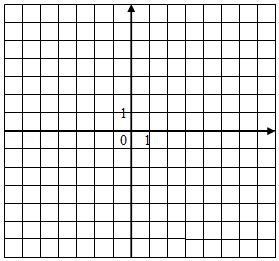
\includegraphics[width=.38\linewidth]{question-24-1.jpg}
\end{center}
\begin{solution}
\textbf{答案：}（Ⅰ）图象见解析；（Ⅱ）$(-\infty,\frac{1}{3})\cup(1,3)\cup(5,+\infty)$

\textbf{分析：}（Ⅰ）运用分段函数的形式写出$f(x)$的解析式，由分段函数的画法，即可得到所求图象；
（Ⅱ）分别讨论当$x\le-1$时，当$-1<x<\frac{3}{2}$时，当$x\ge\frac{3}{2}$时，解绝对值不等式，取交集，最后求并集即可得到所求解集。

\textbf{详解：}（Ⅰ）$f(x)=\begin{cases} x-4, & x\le-1 \\ 3x-2, & -1<x<\frac{3}{2} \\ 4-x, & x\ge\frac{3}{2} \end{cases}$，由分段函数的图象画法，可得$f(x)$的图象，如右；
（Ⅱ）由$|f(x)|>1$，可得当$x\le-1$时，$|x-4|>1$，解得$x>5$或$x<3$，即有$x\le-1$；当$-1<x<\frac{3}{2}$时，$|3x-2|>1$，解得$x>1$或$x<\frac{1}{3}$，即有$-1<x<\frac{1}{3}$或$1<x<\frac{3}{2}$；当$x\ge\frac{3}{2}$时，$|4-x|>1$，解得$x>5$或$x<3$，即有$x>5$或$\frac{3}{2}\le x<3$。综上可得，$x<\frac{1}{3}$或$1<x<3$或$x>5$。则$|f(x)|>1$的解集为$(-\infty,\frac{1}{3})\cup(1,3)\cup(5,+\infty)$。
\end{solution}
\end{question}

